\newpage
\section*{4\quad Order: from sinusoids to rotations (RoPE)}
\addcontentsline{toc}{section}{4 Order: from sinusoids to rotations}
\startchapter{4}
\ifdefined\fitwidthFourFive\else
\newsavebox{\fitboxFourFive}
\newcommand{\fitwidthFourFive}[1]{\sbox{\fitboxFourFive}{\begin{tabular}{@{}c@{}}#1\end{tabular}}\ifdim\wd\fitboxFourFive>\linewidth\resizebox{\linewidth}{!}{\usebox{\fitboxFourFive}}\else\usebox{\fitboxFourFive}\fi}
\fi

\begin{chaptermap}
Chapter 3 ended with a failure: attention cannot tell \tok{waste of time} from \tok{of waste time}. This
chapter gives the model a sense of order. We follow the fixes in the order researchers found them:
learning a vector for each position (GPT-2), adding fixed waves (the 2017 transformer), and finally
rotating the queries and keys by an angle that grows with position (RoPE, used by Qwen3 and most current
models). On the way we prove, with numbers, the property that makes rotation the winner: the score
between two tokens depends only on \emph{how far apart} they are.
\end{chaptermap}

\machine{4}{You are here: Chapter 4 adds the \emph{positions} box on the left. It does not add a new
layer to the stack. It turns each query and key inside attention by an angle that depends on where the
token stands, so attention can finally tell \tok{waste of time} from \tok{of waste time}.}

\begin{beforeyoustart}
(1) A clock's minute hand turns $6^\circ$ per minute. Where is it after 15 minutes?
(2) What are $\cos 0^\circ$, $\cos 90^\circ$ and $\cos 180^\circ$? (3) If you turn an arrow without
stretching it, does its length change? (4) The second hand of a clock and the hour hand both point at
12. Can you tell the time from the second hand alone?

\smallskip\noindent\textit{Refreshers.} (1) $15\times6^\circ = 90^\circ$: pointing at 3. (2) 1, 0 and
$-1$: same direction, right angle, opposite. (3) No; turning keeps the length. (4) No: it repeats every
minute, so you also need the slower hands. Keep this last answer in mind; it is the whole idea of
\S4.6.
\end{beforeyoustart}

%---------------------------------------------------------------------
\subsection*{4.1\quad The failure, once more}

\Predict In Chapter 3 we fed \tok{of waste time} instead of \tok{waste of time}. Before looking back,
guess: did the output for \tok{time} change a lot, a little, or not at all?

Not at all. Both orders give $\bm{o}_{\text{time}} = \nFourNoPosTime$. Look at where order could have entered
the computation. The queries, keys and values are made from each token's own arrow, and the token's
arrow is the same wherever it stands. The score $\bm{q}\cdot\bm{k}$ only sees the two arrows. The mask only
decides which tokens are visible. So to \tok{time}, its past is a bag, as in the bag-of-words attempt of
\S1.4. For a support reply this is serious: \tok{not useful, very good} and \tok{very useful, not good}
would look alike once again.

\begin{wrongidea}{4.1}
``The mask already tells the model the order.'' The mask tells each token \emph{which} tokens it may
see. It says nothing about \emph{where} they stand. It is tempting because the mask is drawn as a triangle
in reading order, so order seems to be built in. But none of $W_Q$, $W_K$, $W_V$ sees a position, and \S4.1
shows it with numbers: same set of earlier tokens, same output.
\end{wrongidea}

\Summary{attention compares arrows that carry no position, so we have to put position into the arrows
ourselves.}

%---------------------------------------------------------------------
\subsection*{4.2\quad Attempt: add a position vector}

\Predict The simplest idea: add the position number to the arrow, so the first token gets $+0$, the
second $+1$, and so on. Can you see a problem with token number 1000?

\Picture Give every seat in a cinema a small badge with its seat number, and pin it onto whoever sits
there. The person is the same; the badge says where they are.

\paragraph{Why plain numbers fail.} If you add $1000$ to every coordinate of the 1000th token, its arrow
is dominated by the badge and the word is lost: $(0,0,1,1)$ becomes $(1000,1000,1001,1001)$, and every
token far into a long text looks the same. The badge has to stay small, and it has to look different at
every position.

\paragraph{Two ways to make good badges.} GPT-2 (Radford and colleagues, 2019) \emph{learned} a table of
badges, one row per position, exactly like the embedding table of Chapter 2: 1024 positions, so it
cannot handle a 1025th token at all. The original transformer (Vaswani and colleagues, 2017) used
\emph{fixed waves} instead. For position $p$ and coordinate pair $i$ (pairs $0,1$; $2,3$; \ldots),
\[
\mathrm{PE}(p, 2i) = \sin\!\Big(\frac{p}{10000^{2i/d}}\Big), \qquad
\mathrm{PE}(p, 2i+1) = \cos\!\Big(\frac{p}{10000^{2i/d}}\Big).
\]
Each pair of coordinates is a wave with its own speed. For our toy, $d=4$ and positions $0,1,2$, so
the badges form a $T\times d = 3\times4$ table, one row per position. Figure~\ref{fig:ch4pe} adds it to
the token arrows, cell by cell.

\begin{center}
\fitwidthFourFive{% AUTO-GENERATED by code/figlib.py helpers -- do not edit
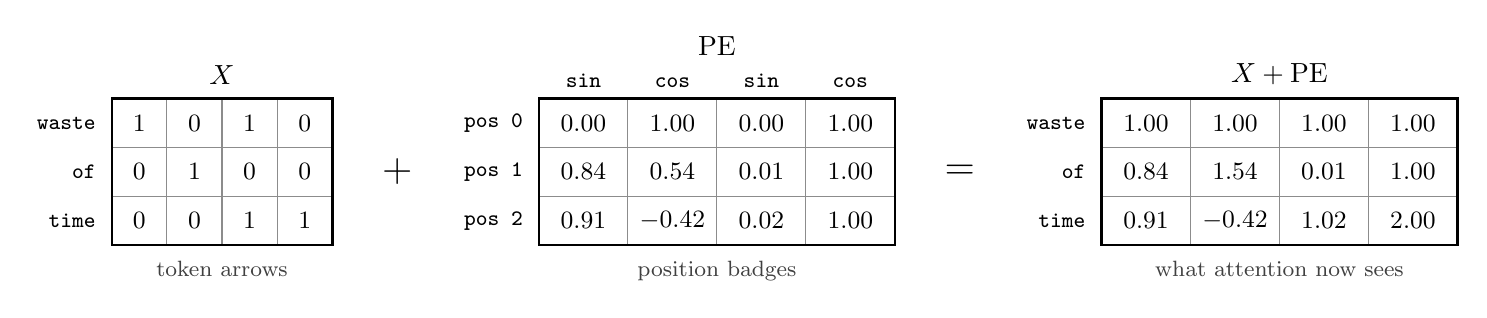
\begin{tikzpicture}
\draw[black!45, fill=white] (0.975,0.930) rectangle (1.675,0.310);
\node[font=\small, text=black] at (1.325,0.620) {$1$};
\draw[black!45, fill=white] (1.675,0.930) rectangle (2.375,0.310);
\node[font=\small, text=black] at (2.025,0.620) {$0$};
\draw[black!45, fill=white] (2.375,0.930) rectangle (3.075,0.310);
\node[font=\small, text=black] at (2.725,0.620) {$1$};
\draw[black!45, fill=white] (3.075,0.930) rectangle (3.775,0.310);
\node[font=\small, text=black] at (3.425,0.620) {$0$};
\draw[black!45, fill=white] (0.975,0.310) rectangle (1.675,-0.310);
\node[font=\small, text=black] at (1.325,-0.000) {$0$};
\draw[black!45, fill=white] (1.675,0.310) rectangle (2.375,-0.310);
\node[font=\small, text=black] at (2.025,-0.000) {$1$};
\draw[black!45, fill=white] (2.375,0.310) rectangle (3.075,-0.310);
\node[font=\small, text=black] at (2.725,-0.000) {$0$};
\draw[black!45, fill=white] (3.075,0.310) rectangle (3.775,-0.310);
\node[font=\small, text=black] at (3.425,-0.000) {$0$};
\draw[black!45, fill=white] (0.975,-0.310) rectangle (1.675,-0.930);
\node[font=\small, text=black] at (1.325,-0.620) {$0$};
\draw[black!45, fill=white] (1.675,-0.310) rectangle (2.375,-0.930);
\node[font=\small, text=black] at (2.025,-0.620) {$0$};
\draw[black!45, fill=white] (2.375,-0.310) rectangle (3.075,-0.930);
\node[font=\small, text=black] at (2.725,-0.620) {$1$};
\draw[black!45, fill=white] (3.075,-0.310) rectangle (3.775,-0.930);
\node[font=\small, text=black] at (3.425,-0.620) {$1$};
\draw[line width=0.9pt] (0.975,0.930) rectangle (3.775,-0.930);
\node[anchor=east, font=\footnotesize\ttfamily] at (0.895,0.620) {waste};
\node[anchor=east, font=\footnotesize\ttfamily] at (0.895,-0.000) {of};
\node[anchor=east, font=\footnotesize\ttfamily] at (0.895,-0.620) {time};
\node[anchor=south, font=\normalsize] at (2.375,0.980) {$X$};
\node[anchor=north, font=\footnotesize, text=black!75] at (2.375,-1.010) {token arrows};
\node[font=\Large] at (4.600,0) {$+$};
\draw[black!45, fill=white] (6.400,0.930) rectangle (7.530,0.310);
\node[font=\small, text=black] at (6.965,0.620) {$0.00$};
\draw[black!45, fill=white] (7.530,0.930) rectangle (8.660,0.310);
\node[font=\small, text=black] at (8.095,0.620) {$1.00$};
\draw[black!45, fill=white] (8.660,0.930) rectangle (9.790,0.310);
\node[font=\small, text=black] at (9.225,0.620) {$0.00$};
\draw[black!45, fill=white] (9.790,0.930) rectangle (10.920,0.310);
\node[font=\small, text=black] at (10.355,0.620) {$1.00$};
\draw[black!45, fill=white] (6.400,0.310) rectangle (7.530,-0.310);
\node[font=\small, text=black] at (6.965,-0.000) {$0.84$};
\draw[black!45, fill=white] (7.530,0.310) rectangle (8.660,-0.310);
\node[font=\small, text=black] at (8.095,-0.000) {$0.54$};
\draw[black!45, fill=white] (8.660,0.310) rectangle (9.790,-0.310);
\node[font=\small, text=black] at (9.225,-0.000) {$0.01$};
\draw[black!45, fill=white] (9.790,0.310) rectangle (10.920,-0.310);
\node[font=\small, text=black] at (10.355,-0.000) {$1.00$};
\draw[black!45, fill=white] (6.400,-0.310) rectangle (7.530,-0.930);
\node[font=\small, text=black] at (6.965,-0.620) {$0.91$};
\draw[black!45, fill=white] (7.530,-0.310) rectangle (8.660,-0.930);
\node[font=\small, text=black] at (8.095,-0.620) {$-0.42$};
\draw[black!45, fill=white] (8.660,-0.310) rectangle (9.790,-0.930);
\node[font=\small, text=black] at (9.225,-0.620) {$0.02$};
\draw[black!45, fill=white] (9.790,-0.310) rectangle (10.920,-0.930);
\node[font=\small, text=black] at (10.355,-0.620) {$1.00$};
\draw[line width=0.9pt] (6.400,0.930) rectangle (10.920,-0.930);
\node[anchor=east, font=\footnotesize\ttfamily] at (6.320,0.620) {pos 0};
\node[anchor=east, font=\footnotesize\ttfamily] at (6.320,-0.000) {pos 1};
\node[anchor=east, font=\footnotesize\ttfamily] at (6.320,-0.620) {pos 2};
\node[anchor=south, font=\footnotesize\ttfamily] at (6.965,0.950) {sin};
\node[anchor=south, font=\footnotesize\ttfamily] at (8.095,0.950) {cos};
\node[anchor=south, font=\footnotesize\ttfamily] at (9.225,0.950) {sin};
\node[anchor=south, font=\footnotesize\ttfamily] at (10.355,0.950) {cos};
\node[anchor=south, font=\normalsize] at (8.660,1.350) {$\mathrm{PE}$};
\node[anchor=north, font=\footnotesize, text=black!75] at (8.660,-1.010) {position badges};
\node[font=\Large] at (11.745,0) {$=$};
\draw[black!45, fill=white] (13.545,0.930) rectangle (14.675,0.310);
\node[font=\small, text=black] at (14.110,0.620) {$1.00$};
\draw[black!45, fill=white] (14.675,0.930) rectangle (15.805,0.310);
\node[font=\small, text=black] at (15.240,0.620) {$1.00$};
\draw[black!45, fill=white] (15.805,0.930) rectangle (16.935,0.310);
\node[font=\small, text=black] at (16.370,0.620) {$1.00$};
\draw[black!45, fill=white] (16.935,0.930) rectangle (18.065,0.310);
\node[font=\small, text=black] at (17.500,0.620) {$1.00$};
\draw[black!45, fill=white] (13.545,0.310) rectangle (14.675,-0.310);
\node[font=\small, text=black] at (14.110,-0.000) {$0.84$};
\draw[black!45, fill=white] (14.675,0.310) rectangle (15.805,-0.310);
\node[font=\small, text=black] at (15.240,-0.000) {$1.54$};
\draw[black!45, fill=white] (15.805,0.310) rectangle (16.935,-0.310);
\node[font=\small, text=black] at (16.370,-0.000) {$0.01$};
\draw[black!45, fill=white] (16.935,0.310) rectangle (18.065,-0.310);
\node[font=\small, text=black] at (17.500,-0.000) {$1.00$};
\draw[black!45, fill=white] (13.545,-0.310) rectangle (14.675,-0.930);
\node[font=\small, text=black] at (14.110,-0.620) {$0.91$};
\draw[black!45, fill=white] (14.675,-0.310) rectangle (15.805,-0.930);
\node[font=\small, text=black] at (15.240,-0.620) {$-0.42$};
\draw[black!45, fill=white] (15.805,-0.310) rectangle (16.935,-0.930);
\node[font=\small, text=black] at (16.370,-0.620) {$1.02$};
\draw[black!45, fill=white] (16.935,-0.310) rectangle (18.065,-0.930);
\node[font=\small, text=black] at (17.500,-0.620) {$2.00$};
\draw[line width=0.9pt] (13.545,0.930) rectangle (18.065,-0.930);
\node[anchor=east, font=\footnotesize\ttfamily] at (13.465,0.620) {waste};
\node[anchor=east, font=\footnotesize\ttfamily] at (13.465,-0.000) {of};
\node[anchor=east, font=\footnotesize\ttfamily] at (13.465,-0.620) {time};
\node[anchor=south, font=\normalsize] at (15.805,0.980) {$X+\mathrm{PE}$};
\node[anchor=north, font=\footnotesize, text=black!75] at (15.805,-1.010) {what attention now sees};
\end{tikzpicture}
}
\captionof{figure}{Sinusoidal badges as a matrix. Row $p$ of $\mathrm{PE}$ is the badge for position $p$; it is
added to the token arrow in the same row. Notice the second pair of columns barely changes from row to
row (it is the slow wave), while the first pair changes a lot (the fast wave).}
\label{fig:ch4pe}
\end{center}

Every entry of $\mathrm{PE}$ stays between $-1$ and $1$, however long the text. Add these badges to the toy arrows and run
the attention of Chapter 3 again. \tok{time}'s output becomes $\nFourSinTime$ for \tok{waste of time} and
$\nFourSinTimeSwap$ for \tok{of waste time}. The two orders now differ (by up to \nFourSinDiff\ in one
coordinate). Requirement 2 is back.

\begin{figure}[h]
\centering
\begin{tikzpicture}
\begin{axis}[width=12cm, height=4.2cm, xlabel={position $p$}, ylabel={value},
  xlabel style={font=\small}, ylabel style={font=\small}, tick label style={font=\small},
  axis lines*=left, ymin=-1.15, ymax=1.15, xmin=0, xmax=40, legend style={font=\footnotesize, draw=none, at={(0.5,1.03)}, anchor=south}, legend columns=3]
\addplot[black, thick] table[x=pos, y=fast] {data_ch4/waves.dat};
\addplot[black!60, very thick, densely dotted] table[x=pos, y=mid] {data_ch4/waves.dat};
\addplot[black!70, thick, dashed] table[x=pos, y=slow] {data_ch4/waves.dat};
\legend{pair 0 (repeats every \nFourWlMin), pair 4 (every \nFourMidWl), pair 8 (every \nFourSlowWl)}
\end{axis}
\end{tikzpicture}
\caption{Three of the waves used for $d=64$: solid is fast, dotted is medium, dashed is slow. Fast waves tell neighbours apart; slow waves tell far
positions apart. For $d=64$ the repeat lengths run from \nFourWlMin\ to \nFourWlMax\ positions.}
\end{figure}

\begin{wrongidea}{4.2}
``Add the position number itself.'' The number grows without limit and swamps the word. A useful badge
has two properties at once: it stays small, and it is different at every position. Waves have both.
\end{wrongidea}

\begin{breaks}
A badge is pinned on and stays separate from the person. Here the badge is \emph{added} into the same
numbers as the word, so the model receives a single blended arrow and must learn to pull the two apart.
That blending is the weakness the next fix removes.
\end{breaks}

\Summary{adding a small, position-specific vector to each arrow restores order, as long as the vector
stays bounded and differs from position to position.}

%---------------------------------------------------------------------
\subsection*{4.3\quad What should position mean? Absolute or relative}

Tell me: in \tok{waste of time}, what matters to \tok{time} about \tok{waste}? That \tok{waste} is word
number 0 of the message, or that it is two words back? Put the same three words in the middle of a long
complaint and \tok{waste} might be word 340. Nothing about the meaning has changed. What stayed the same
is the \emph{distance}: two words back.

Added badges mix this up. The score between \tok{time} and \tok{waste} becomes a dot product of
(word + badge) with (word + badge), which contains word-badge cross terms that depend on the absolute
positions. The model can learn to undo this, but we are asking it to do extra work. Shaw, Uszkoreit and
Vaswani (2018) proposed putting the \emph{distance} directly into attention. Su and colleagues (2021)
found an elegant way to do it with no extra table at all: rotation.

\begin{wrongidea}{4.3}
``Positions have to be learned, like every other weight.'' It is tempting because almost everything else in
the model is learned. Learning them (GPT-2) is one option. The sinusoids of \S4.2 and the rotations of \S4.4
are fixed formulas with nothing to learn, and they work for positions never seen in training.
\end{wrongidea}

\Summary{what usually matters is how far apart two tokens are, so a good position method should make the
score depend on distance.}

%---------------------------------------------------------------------
\subsection*{4.4\quad The fix: rotate the questions and the labels}

\Predict If you turn two arrows by the \emph{same} angle, does the angle between them change? If you turn
one by $30^\circ$ and the other by $50^\circ$, what is the angle between them now, compared with before?

\Picture A clock. Split each query and key into pairs of numbers, and draw each pair as a clock hand.
A token at position $p$ has each of its hands turned forward by $p$ ticks. Turning both hands of a pair by
the same amount leaves their angle unchanged; only the \emph{difference} in ticks shows up between them.
That is exactly ``how far apart''.

\begin{figure}[h]
\centering
\begin{tikzpicture}[scale=1.3, font=\small]
\draw[gray!60] (-1.6,0)--(1.6,0); \draw[gray!40] (0,-0.3)--(0,1.6);
\draw[-{Stealth}, thick] (0,0) -- (1.4,0) node[below right] {$\bm{k}$ at position $n$};
\draw[-{Stealth}, very thick, black!65] (0,0) -- (0.70,1.21) node[above right] {$\bm{q}$ at position $m$};
\draw (0.45,0) arc[start angle=0, end angle=60, radius=0.45]; \node at (0.66,0.3) {$\varphi$};
\begin{scope}[xshift=6.2cm]
\draw[gray!60] (-1.6,0)--(1.6,0); \draw[gray!60] (0,-0.3)--(0,1.6);
\draw[-{Stealth}, thick] (0,0) -- (1.21,0.70) node[right] {$\bm{k}$ turned by $n\theta$};
\draw[-{Stealth}, very thick, black!65] (0,0) -- (-0.48,1.32) node[above left] {$\bm{q}$ turned by $m\theta$};
\draw (0.39,0.225) arc[start angle=30, end angle=110, radius=0.45];
\node[align=left] at (1.05,1.05) {$\varphi + (m-n)\theta$};
\end{scope}
\end{tikzpicture}
\caption{Rotary position embedding on one pair of coordinates. Each arrow is turned by its own position
times $\theta$. The angle between them changes by $(m-n)\theta$, which depends only on the distance.}
\end{figure}

\paragraph{The numbers.} Our toy has $d_k=4$, so two pairs: coordinates $(1,2)$ and $(3,4)$. RoPE turns pair
$i$ by $p\,\theta_i$ at position $p$, with $\theta_i = b^{-2i/d}$ for a chosen base $b$. Real models use
$b=10{,}000$ or more. With $d=4$ that makes the second pair turn by only \nFourBigThetaTwo\ radians per
position, too slow to see in a three-word example (the shares barely move:
$\nFourBigBaseA$). So for the toy we use $b=4$, which gives $\theta = (\nFourThetaOne,\ \nFourThetaTwo)$
radians per position: the first hand turns \nFourDegOne$^\circ$ per word, the second \nFourDegTwo$^\circ$.

How does a turn act on numbers? It is a $2\times2$ matrix multiplying one pair. Take \tok{time}'s query,
$(0,0,1,1)$, at position 2. Its second pair is $(1,1)$ and must turn by $2\theta_2 = 2\times\nFourThetaTwo = 1$
radian. Figure~\ref{fig:ch4rot} does that multiplication.

\begin{center}
\fitwidthFourFive{% AUTO-GENERATED by code/figlib.py helpers -- do not edit
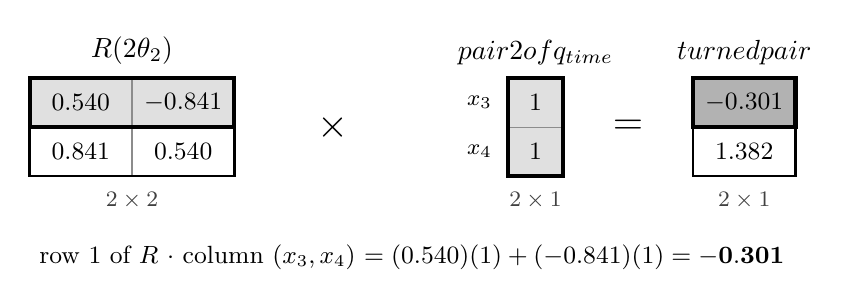
\begin{tikzpicture}
\draw[black!45, fill=black!12] (0.000,0.620) rectangle (1.300,0.000);
\node[font=\small, text=black] at (0.650,0.310) {$0.540$};
\draw[black!45, fill=black!12] (1.300,0.620) rectangle (2.600,0.000);
\node[font=\small, text=black] at (1.950,0.310) {$-0.841$};
\draw[black!45, fill=white] (0.000,0.000) rectangle (1.300,-0.620);
\node[font=\small, text=black] at (0.650,-0.310) {$0.841$};
\draw[black!45, fill=white] (1.300,0.000) rectangle (2.600,-0.620);
\node[font=\small, text=black] at (1.950,-0.310) {$0.540$};
\draw[line width=1.4pt] (0.000,0.620) rectangle (2.600,0.000);
\draw[line width=0.9pt] (0.000,0.620) rectangle (2.600,-0.620);
\node[anchor=south, font=\normalsize] at (1.300,0.670) {$R(2\theta_2)$};
\node[anchor=north, font=\footnotesize, text=black!75] at (1.300,-0.700) {$2\times2$};
\node[font=\Large] at (3.850,0) {$\times$};
\draw[black!45, fill=black!12] (6.075,0.620) rectangle (6.775,0.000);
\node[font=\small, text=black] at (6.425,0.310) {$1$};
\draw[black!45, fill=black!12] (6.075,0.000) rectangle (6.775,-0.620);
\node[font=\small, text=black] at (6.425,-0.310) {$1$};
\draw[line width=1.4pt] (6.075,0.620) rectangle (6.775,-0.620);
\draw[line width=0.9pt] (6.075,0.620) rectangle (6.775,-0.620);
\node[anchor=east, font=\footnotesize\ttfamily] at (5.995,0.310) {$x_3$};
\node[anchor=east, font=\footnotesize\ttfamily] at (5.995,-0.310) {$x_4$};
\node[anchor=south, font=\normalsize] at (6.425,0.670) {$\text{pair 2 of }\bm q_{\text{time}}$};
\node[anchor=north, font=\footnotesize, text=black!75] at (6.425,-0.700) {$2\times1$};
\node[font=\Large] at (7.600,0) {$=$};
\draw[black!45, fill=black!30] (8.425,0.620) rectangle (9.725,0.000);
\node[font=\small, text=black] at (9.075,0.310) {$-0.301$};
\draw[black!45, fill=white] (8.425,0.000) rectangle (9.725,-0.620);
\node[font=\small, text=black] at (9.075,-0.310) {$1.382$};
\draw[line width=1.6pt] (8.425,0.620) rectangle (9.725,0.000);
\draw[line width=0.9pt] (8.425,0.620) rectangle (9.725,-0.620);
\node[anchor=south, font=\normalsize] at (9.075,0.670) {$\text{turned pair}$};
\node[anchor=north, font=\footnotesize, text=black!75] at (9.075,-0.700) {$2\times1$};
\node[anchor=north west, font=\small, align=left] at (0,-1.370) {row 1 of $R$ $\cdot$ column $(x_3, x_4)$ $= (0.540)(1) + (-0.841)(1) = \mathbf{-0.301}$};
\end{tikzpicture}
}
\captionof{figure}{One turn, as a matrix product. Row 1 of the rotation matrix meets the pair $(x_3,x_4)=(1,1)$ and
gives the first number of the turned pair. The second row gives the second number the same way. The
pair's length is $\sqrt2$ before and after.}
\label{fig:ch4rot}
\end{center}

Only queries and keys are turned; values are left alone. Do the same for every pair of every row, each
row by its own position, and you get Figure~\ref{fig:ch4qk}. \tok{waste} sits at position 0, so its row is
not turned at all.

\begin{center}
\fitwidthFourFive{% AUTO-GENERATED by code/figlib.py helpers -- do not edit
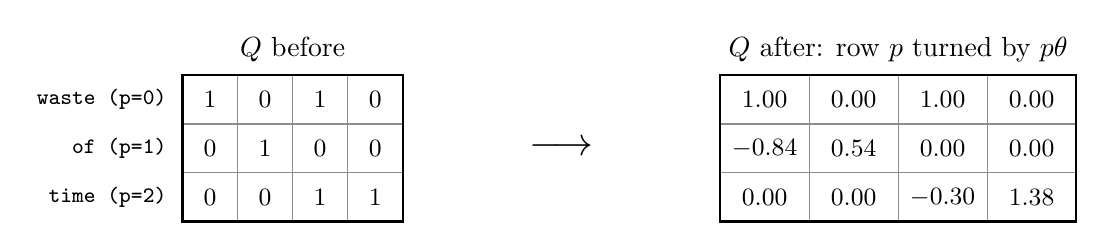
\begin{tikzpicture}
\draw[black!45, fill=white] (1.965,0.930) rectangle (2.665,0.310);
\node[font=\small, text=black] at (2.315,0.620) {$1$};
\draw[black!45, fill=white] (2.665,0.930) rectangle (3.365,0.310);
\node[font=\small, text=black] at (3.015,0.620) {$0$};
\draw[black!45, fill=white] (3.365,0.930) rectangle (4.065,0.310);
\node[font=\small, text=black] at (3.715,0.620) {$1$};
\draw[black!45, fill=white] (4.065,0.930) rectangle (4.765,0.310);
\node[font=\small, text=black] at (4.415,0.620) {$0$};
\draw[black!45, fill=white] (1.965,0.310) rectangle (2.665,-0.310);
\node[font=\small, text=black] at (2.315,-0.000) {$0$};
\draw[black!45, fill=white] (2.665,0.310) rectangle (3.365,-0.310);
\node[font=\small, text=black] at (3.015,-0.000) {$1$};
\draw[black!45, fill=white] (3.365,0.310) rectangle (4.065,-0.310);
\node[font=\small, text=black] at (3.715,-0.000) {$0$};
\draw[black!45, fill=white] (4.065,0.310) rectangle (4.765,-0.310);
\node[font=\small, text=black] at (4.415,-0.000) {$0$};
\draw[black!45, fill=white] (1.965,-0.310) rectangle (2.665,-0.930);
\node[font=\small, text=black] at (2.315,-0.620) {$0$};
\draw[black!45, fill=white] (2.665,-0.310) rectangle (3.365,-0.930);
\node[font=\small, text=black] at (3.015,-0.620) {$0$};
\draw[black!45, fill=white] (3.365,-0.310) rectangle (4.065,-0.930);
\node[font=\small, text=black] at (3.715,-0.620) {$1$};
\draw[black!45, fill=white] (4.065,-0.310) rectangle (4.765,-0.930);
\node[font=\small, text=black] at (4.415,-0.620) {$1$};
\draw[line width=0.9pt] (1.965,0.930) rectangle (4.765,-0.930);
\node[anchor=east, font=\footnotesize\ttfamily] at (1.885,0.620) {waste (p=0)};
\node[anchor=east, font=\footnotesize\ttfamily] at (1.885,-0.000) {of (p=1)};
\node[anchor=east, font=\footnotesize\ttfamily] at (1.885,-0.620) {time (p=2)};
\node[anchor=south, font=\normalsize] at (3.365,0.980) {$Q$ before};
\node[font=\Large] at (6.780,0) {$\longrightarrow$};
\draw[black!45, fill=white] (8.795,0.930) rectangle (9.925,0.310);
\node[font=\small, text=black] at (9.360,0.620) {$1.00$};
\draw[black!45, fill=white] (9.925,0.930) rectangle (11.055,0.310);
\node[font=\small, text=black] at (10.490,0.620) {$0.00$};
\draw[black!45, fill=white] (11.055,0.930) rectangle (12.185,0.310);
\node[font=\small, text=black] at (11.620,0.620) {$1.00$};
\draw[black!45, fill=white] (12.185,0.930) rectangle (13.315,0.310);
\node[font=\small, text=black] at (12.750,0.620) {$0.00$};
\draw[black!45, fill=white] (8.795,0.310) rectangle (9.925,-0.310);
\node[font=\small, text=black] at (9.360,-0.000) {$-0.84$};
\draw[black!45, fill=white] (9.925,0.310) rectangle (11.055,-0.310);
\node[font=\small, text=black] at (10.490,-0.000) {$0.54$};
\draw[black!45, fill=white] (11.055,0.310) rectangle (12.185,-0.310);
\node[font=\small, text=black] at (11.620,-0.000) {$0.00$};
\draw[black!45, fill=white] (12.185,0.310) rectangle (13.315,-0.310);
\node[font=\small, text=black] at (12.750,-0.000) {$0.00$};
\draw[black!45, fill=white] (8.795,-0.310) rectangle (9.925,-0.930);
\node[font=\small, text=black] at (9.360,-0.620) {$0.00$};
\draw[black!45, fill=white] (9.925,-0.310) rectangle (11.055,-0.930);
\node[font=\small, text=black] at (10.490,-0.620) {$0.00$};
\draw[black!45, fill=white] (11.055,-0.310) rectangle (12.185,-0.930);
\node[font=\small, text=black] at (11.620,-0.620) {$-0.30$};
\draw[black!45, fill=white] (12.185,-0.310) rectangle (13.315,-0.930);
\node[font=\small, text=black] at (12.750,-0.620) {$1.38$};
\draw[line width=0.9pt] (8.795,0.930) rectangle (13.315,-0.930);
\node[anchor=south, font=\normalsize] at (11.055,0.980) {$Q$ after: row $p$ turned by $p\theta$};
\end{tikzpicture}
\\[10pt]
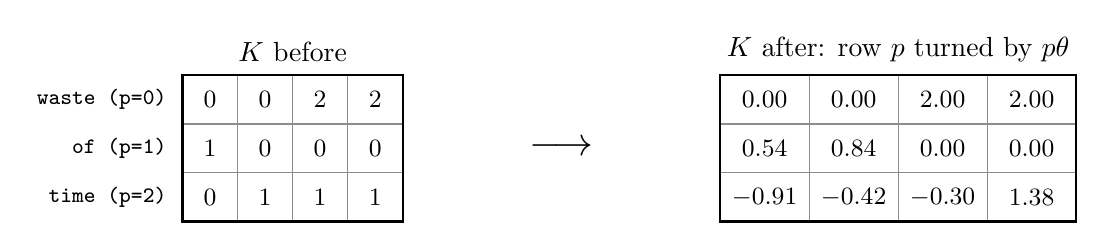
\begin{tikzpicture}
\draw[black!45, fill=white] (1.965,0.930) rectangle (2.665,0.310);
\node[font=\small, text=black] at (2.315,0.620) {$0$};
\draw[black!45, fill=white] (2.665,0.930) rectangle (3.365,0.310);
\node[font=\small, text=black] at (3.015,0.620) {$0$};
\draw[black!45, fill=white] (3.365,0.930) rectangle (4.065,0.310);
\node[font=\small, text=black] at (3.715,0.620) {$2$};
\draw[black!45, fill=white] (4.065,0.930) rectangle (4.765,0.310);
\node[font=\small, text=black] at (4.415,0.620) {$2$};
\draw[black!45, fill=white] (1.965,0.310) rectangle (2.665,-0.310);
\node[font=\small, text=black] at (2.315,-0.000) {$1$};
\draw[black!45, fill=white] (2.665,0.310) rectangle (3.365,-0.310);
\node[font=\small, text=black] at (3.015,-0.000) {$0$};
\draw[black!45, fill=white] (3.365,0.310) rectangle (4.065,-0.310);
\node[font=\small, text=black] at (3.715,-0.000) {$0$};
\draw[black!45, fill=white] (4.065,0.310) rectangle (4.765,-0.310);
\node[font=\small, text=black] at (4.415,-0.000) {$0$};
\draw[black!45, fill=white] (1.965,-0.310) rectangle (2.665,-0.930);
\node[font=\small, text=black] at (2.315,-0.620) {$0$};
\draw[black!45, fill=white] (2.665,-0.310) rectangle (3.365,-0.930);
\node[font=\small, text=black] at (3.015,-0.620) {$1$};
\draw[black!45, fill=white] (3.365,-0.310) rectangle (4.065,-0.930);
\node[font=\small, text=black] at (3.715,-0.620) {$1$};
\draw[black!45, fill=white] (4.065,-0.310) rectangle (4.765,-0.930);
\node[font=\small, text=black] at (4.415,-0.620) {$1$};
\draw[line width=0.9pt] (1.965,0.930) rectangle (4.765,-0.930);
\node[anchor=east, font=\footnotesize\ttfamily] at (1.885,0.620) {waste (p=0)};
\node[anchor=east, font=\footnotesize\ttfamily] at (1.885,-0.000) {of (p=1)};
\node[anchor=east, font=\footnotesize\ttfamily] at (1.885,-0.620) {time (p=2)};
\node[anchor=south, font=\normalsize] at (3.365,0.980) {$K$ before};
\node[font=\Large] at (6.780,0) {$\longrightarrow$};
\draw[black!45, fill=white] (8.795,0.930) rectangle (9.925,0.310);
\node[font=\small, text=black] at (9.360,0.620) {$0.00$};
\draw[black!45, fill=white] (9.925,0.930) rectangle (11.055,0.310);
\node[font=\small, text=black] at (10.490,0.620) {$0.00$};
\draw[black!45, fill=white] (11.055,0.930) rectangle (12.185,0.310);
\node[font=\small, text=black] at (11.620,0.620) {$2.00$};
\draw[black!45, fill=white] (12.185,0.930) rectangle (13.315,0.310);
\node[font=\small, text=black] at (12.750,0.620) {$2.00$};
\draw[black!45, fill=white] (8.795,0.310) rectangle (9.925,-0.310);
\node[font=\small, text=black] at (9.360,-0.000) {$0.54$};
\draw[black!45, fill=white] (9.925,0.310) rectangle (11.055,-0.310);
\node[font=\small, text=black] at (10.490,-0.000) {$0.84$};
\draw[black!45, fill=white] (11.055,0.310) rectangle (12.185,-0.310);
\node[font=\small, text=black] at (11.620,-0.000) {$0.00$};
\draw[black!45, fill=white] (12.185,0.310) rectangle (13.315,-0.310);
\node[font=\small, text=black] at (12.750,-0.000) {$0.00$};
\draw[black!45, fill=white] (8.795,-0.310) rectangle (9.925,-0.930);
\node[font=\small, text=black] at (9.360,-0.620) {$-0.91$};
\draw[black!45, fill=white] (9.925,-0.310) rectangle (11.055,-0.930);
\node[font=\small, text=black] at (10.490,-0.620) {$-0.42$};
\draw[black!45, fill=white] (11.055,-0.310) rectangle (12.185,-0.930);
\node[font=\small, text=black] at (11.620,-0.620) {$-0.30$};
\draw[black!45, fill=white] (12.185,-0.310) rectangle (13.315,-0.930);
\node[font=\small, text=black] at (12.750,-0.620) {$1.38$};
\draw[line width=0.9pt] (8.795,0.930) rectangle (13.315,-0.930);
\node[anchor=south, font=\normalsize] at (11.055,0.980) {$K$ after: row $p$ turned by $p\theta$};
\end{tikzpicture}
}
\captionof{figure}{Queries and keys of \tok{waste of time} before and after RoPE. Row $p$ is turned by $p$ times
$\theta$ (both of its pairs, each with its own speed). Row \tok{waste} ($p=0$) is unchanged.}
\label{fig:ch4qk}
\end{center}

\noindent Read the last row of $Q$ after turning: that is \tok{time}'s turned query. Now swap the first two words: \tok{waste}
moves to position 1, one step from \tok{time} instead of two. Figure~\ref{fig:ch4scores} shows the
whole score table $QK^\top$ (before scaling) for both orders, without and with RoPE.

\begin{center}
\fitwidthFourFive{% AUTO-GENERATED by code/figlib.py helpers -- do not edit
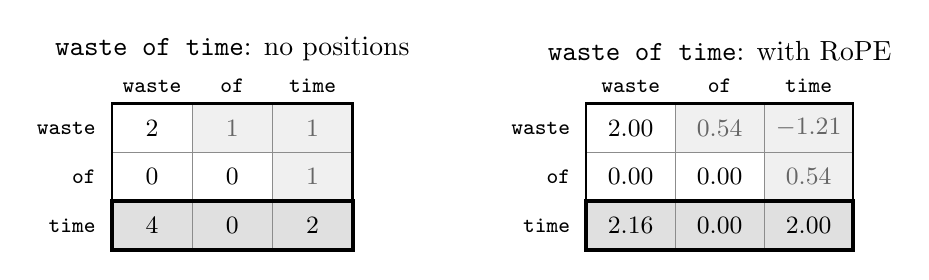
\begin{tikzpicture}
\draw[black!45, fill=white] (0.975,0.930) rectangle (1.995,0.310);
\node[font=\small, text=black] at (1.485,0.620) {$2$};
\draw[black!45, fill=black!6] (1.995,0.930) rectangle (3.015,0.310);
\node[font=\small, text=black!60] at (2.505,0.620) {$1$};
\draw[black!45, fill=black!6] (3.015,0.930) rectangle (4.035,0.310);
\node[font=\small, text=black!60] at (3.525,0.620) {$1$};
\draw[black!45, fill=white] (0.975,0.310) rectangle (1.995,-0.310);
\node[font=\small, text=black] at (1.485,-0.000) {$0$};
\draw[black!45, fill=white] (1.995,0.310) rectangle (3.015,-0.310);
\node[font=\small, text=black] at (2.505,-0.000) {$0$};
\draw[black!45, fill=black!6] (3.015,0.310) rectangle (4.035,-0.310);
\node[font=\small, text=black!60] at (3.525,-0.000) {$1$};
\draw[black!45, fill=black!12] (0.975,-0.310) rectangle (1.995,-0.930);
\node[font=\small, text=black] at (1.485,-0.620) {$4$};
\draw[black!45, fill=black!12] (1.995,-0.310) rectangle (3.015,-0.930);
\node[font=\small, text=black] at (2.505,-0.620) {$0$};
\draw[black!45, fill=black!12] (3.015,-0.310) rectangle (4.035,-0.930);
\node[font=\small, text=black] at (3.525,-0.620) {$2$};
\draw[line width=1.4pt] (0.975,-0.310) rectangle (4.035,-0.930);
\draw[line width=0.9pt] (0.975,0.930) rectangle (4.035,-0.930);
\node[anchor=east, font=\footnotesize\ttfamily] at (0.895,0.620) {waste};
\node[anchor=east, font=\footnotesize\ttfamily] at (0.895,-0.000) {of};
\node[anchor=east, font=\footnotesize\ttfamily] at (0.895,-0.620) {time};
\node[anchor=south, font=\footnotesize\ttfamily] at (1.485,0.950) {waste};
\node[anchor=south, font=\footnotesize\ttfamily] at (2.505,0.950) {of};
\node[anchor=south, font=\footnotesize\ttfamily] at (3.525,0.950) {time};
\node[anchor=south, font=\normalsize] at (2.505,1.350) {\texttt{waste of time}: no positions};
\node[font=\Large] at (5.030,0) {\quad};
\draw[black!45, fill=white] (7.000,0.930) rectangle (8.130,0.310);
\node[font=\small, text=black] at (7.565,0.620) {$2.00$};
\draw[black!45, fill=black!6] (8.130,0.930) rectangle (9.260,0.310);
\node[font=\small, text=black!60] at (8.695,0.620) {$0.54$};
\draw[black!45, fill=black!6] (9.260,0.930) rectangle (10.390,0.310);
\node[font=\small, text=black!60] at (9.825,0.620) {$-1.21$};
\draw[black!45, fill=white] (7.000,0.310) rectangle (8.130,-0.310);
\node[font=\small, text=black] at (7.565,-0.000) {$0.00$};
\draw[black!45, fill=white] (8.130,0.310) rectangle (9.260,-0.310);
\node[font=\small, text=black] at (8.695,-0.000) {$0.00$};
\draw[black!45, fill=black!6] (9.260,0.310) rectangle (10.390,-0.310);
\node[font=\small, text=black!60] at (9.825,-0.000) {$0.54$};
\draw[black!45, fill=black!12] (7.000,-0.310) rectangle (8.130,-0.930);
\node[font=\small, text=black] at (7.565,-0.620) {$2.16$};
\draw[black!45, fill=black!12] (8.130,-0.310) rectangle (9.260,-0.930);
\node[font=\small, text=black] at (8.695,-0.620) {$0.00$};
\draw[black!45, fill=black!12] (9.260,-0.310) rectangle (10.390,-0.930);
\node[font=\small, text=black] at (9.825,-0.620) {$2.00$};
\draw[line width=1.4pt] (7.000,-0.310) rectangle (10.390,-0.930);
\draw[line width=0.9pt] (7.000,0.930) rectangle (10.390,-0.930);
\node[anchor=east, font=\footnotesize\ttfamily] at (6.920,0.620) {waste};
\node[anchor=east, font=\footnotesize\ttfamily] at (6.920,-0.000) {of};
\node[anchor=east, font=\footnotesize\ttfamily] at (6.920,-0.620) {time};
\node[anchor=south, font=\footnotesize\ttfamily] at (7.565,0.950) {waste};
\node[anchor=south, font=\footnotesize\ttfamily] at (8.695,0.950) {of};
\node[anchor=south, font=\footnotesize\ttfamily] at (9.825,0.950) {time};
\node[anchor=south, font=\normalsize] at (8.695,1.350) {\texttt{waste of time}: with RoPE};
\end{tikzpicture}
\\[10pt]
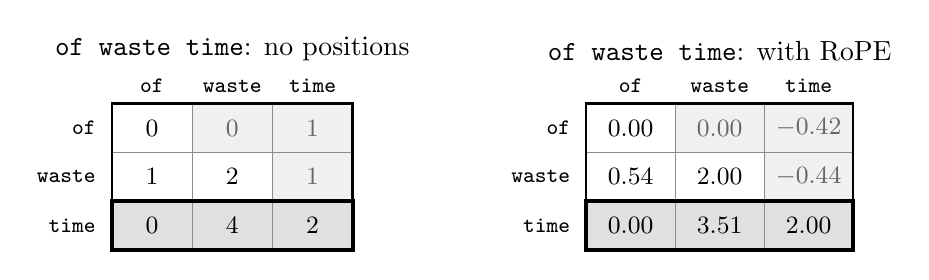
\begin{tikzpicture}
\draw[black!45, fill=white] (0.975,0.930) rectangle (1.995,0.310);
\node[font=\small, text=black] at (1.485,0.620) {$0$};
\draw[black!45, fill=black!6] (1.995,0.930) rectangle (3.015,0.310);
\node[font=\small, text=black!60] at (2.505,0.620) {$0$};
\draw[black!45, fill=black!6] (3.015,0.930) rectangle (4.035,0.310);
\node[font=\small, text=black!60] at (3.525,0.620) {$1$};
\draw[black!45, fill=white] (0.975,0.310) rectangle (1.995,-0.310);
\node[font=\small, text=black] at (1.485,-0.000) {$1$};
\draw[black!45, fill=white] (1.995,0.310) rectangle (3.015,-0.310);
\node[font=\small, text=black] at (2.505,-0.000) {$2$};
\draw[black!45, fill=black!6] (3.015,0.310) rectangle (4.035,-0.310);
\node[font=\small, text=black!60] at (3.525,-0.000) {$1$};
\draw[black!45, fill=black!12] (0.975,-0.310) rectangle (1.995,-0.930);
\node[font=\small, text=black] at (1.485,-0.620) {$0$};
\draw[black!45, fill=black!12] (1.995,-0.310) rectangle (3.015,-0.930);
\node[font=\small, text=black] at (2.505,-0.620) {$4$};
\draw[black!45, fill=black!12] (3.015,-0.310) rectangle (4.035,-0.930);
\node[font=\small, text=black] at (3.525,-0.620) {$2$};
\draw[line width=1.4pt] (0.975,-0.310) rectangle (4.035,-0.930);
\draw[line width=0.9pt] (0.975,0.930) rectangle (4.035,-0.930);
\node[anchor=east, font=\footnotesize\ttfamily] at (0.895,0.620) {of};
\node[anchor=east, font=\footnotesize\ttfamily] at (0.895,-0.000) {waste};
\node[anchor=east, font=\footnotesize\ttfamily] at (0.895,-0.620) {time};
\node[anchor=south, font=\footnotesize\ttfamily] at (1.485,0.950) {of};
\node[anchor=south, font=\footnotesize\ttfamily] at (2.505,0.950) {waste};
\node[anchor=south, font=\footnotesize\ttfamily] at (3.525,0.950) {time};
\node[anchor=south, font=\normalsize] at (2.505,1.350) {\texttt{of waste time}: no positions};
\node[font=\Large] at (5.030,0) {\quad};
\draw[black!45, fill=white] (7.000,0.930) rectangle (8.130,0.310);
\node[font=\small, text=black] at (7.565,0.620) {$0.00$};
\draw[black!45, fill=black!6] (8.130,0.930) rectangle (9.260,0.310);
\node[font=\small, text=black!60] at (8.695,0.620) {$0.00$};
\draw[black!45, fill=black!6] (9.260,0.930) rectangle (10.390,0.310);
\node[font=\small, text=black!60] at (9.825,0.620) {$-0.42$};
\draw[black!45, fill=white] (7.000,0.310) rectangle (8.130,-0.310);
\node[font=\small, text=black] at (7.565,-0.000) {$0.54$};
\draw[black!45, fill=white] (8.130,0.310) rectangle (9.260,-0.310);
\node[font=\small, text=black] at (8.695,-0.000) {$2.00$};
\draw[black!45, fill=black!6] (9.260,0.310) rectangle (10.390,-0.310);
\node[font=\small, text=black!60] at (9.825,-0.000) {$-0.44$};
\draw[black!45, fill=black!12] (7.000,-0.310) rectangle (8.130,-0.930);
\node[font=\small, text=black] at (7.565,-0.620) {$0.00$};
\draw[black!45, fill=black!12] (8.130,-0.310) rectangle (9.260,-0.930);
\node[font=\small, text=black] at (8.695,-0.620) {$3.51$};
\draw[black!45, fill=black!12] (9.260,-0.310) rectangle (10.390,-0.930);
\node[font=\small, text=black] at (9.825,-0.620) {$2.00$};
\draw[line width=1.4pt] (7.000,-0.310) rectangle (10.390,-0.930);
\draw[line width=0.9pt] (7.000,0.930) rectangle (10.390,-0.930);
\node[anchor=east, font=\footnotesize\ttfamily] at (6.920,0.620) {of};
\node[anchor=east, font=\footnotesize\ttfamily] at (6.920,-0.000) {waste};
\node[anchor=east, font=\footnotesize\ttfamily] at (6.920,-0.620) {time};
\node[anchor=south, font=\footnotesize\ttfamily] at (7.565,0.950) {of};
\node[anchor=south, font=\footnotesize\ttfamily] at (8.695,0.950) {waste};
\node[anchor=south, font=\footnotesize\ttfamily] at (9.825,0.950) {time};
\node[anchor=south, font=\normalsize] at (8.695,1.350) {\texttt{of waste time}: with RoPE};
\end{tikzpicture}
}
\captionof{figure}{Score tables for both word orders. Grey cells are covered by the causal mask. Compare the
outlined \tok{time} rows. Without positions they hold the same three numbers, only reordered: \tok{waste}
scores 4 wherever it stands. With RoPE \tok{waste}'s score depends on how far it is from \tok{time}.}
\label{fig:ch4scores}
\end{center}

\noindent For the query \tok{time}, after scaling and softmax:
\begin{center}
\small
\begin{tabular}{@{}l l l l@{}}
\toprule
order & dot products (before scaling) & shares after softmax & output $\bm{o}_{\text{time}}$\\
\midrule
\tok{waste of time} & $\nFourRopeScores$ & $\nFourRopeA$ & $\nFourRopeTime$\\
\tok{of waste time} & $\nFourRopeScoresSwap$ & $\nFourRopeASwap$ & $\nFourRopeTimeSwap$\\
\bottomrule
\end{tabular}
\end{center}
Each row lists the tokens in sentence order. \tok{waste}'s share goes from \nFourOrigWaste\ to
\nFourSwapWaste\ when it moves closer. Order now changes the answer, and nothing was added to any arrow:
the script checks that every turned arrow keeps its length.

\Exactly For a pair $(x_1, x_2)$ at position $p$, RoPE applies the rotation
\[
\begin{pmatrix} x_1' \\ x_2' \end{pmatrix} =
\begin{pmatrix} \cos p\theta & -\sin p\theta \\ \sin p\theta & \cos p\theta \end{pmatrix}
\begin{pmatrix} x_1 \\ x_2 \end{pmatrix},
\]
to every pair of every query and key, each pair with its own $\theta_i$. Write $R_p$ for this rotation.
Because turning by $m\theta$ and then measuring against something turned by $n\theta$ is the same as
turning by $(m-n)\theta$ alone,
\[
(R_m\bm{q})\cdot(R_n\bm{k}) \;=\; \bm{q}\cdot(R_{n-m}\bm{k}),
\]
which depends on $m$ and $n$ only through $m-n$. We checked this numerically on 1000 random queries and
keys of width 8 at random positions, shifting both positions by the same amount: the largest difference
in score was $\nFourRelWorst$, which is rounding error. In the toy, \tok{time} at position 2 looking at
\tok{waste} at 0 scores \nFourRelScore, and so does \tok{time} at 7 looking at \tok{waste} at 5.

\begin{wrongidea}{4.4}
``RoPE changes the token's embedding.'' It does not touch the embedding table or the values. It turns
the query and key after $W_Q$ and $W_K$ have made them, inside every attention layer, and it never changes
their length. What a token hands over (its value) is the same wherever it stands; only \emph{who finds
it} depends on distance.
\end{wrongidea}

\begin{checkq}
After RoPE, \tok{time} at position 2 and \tok{waste} at position 0 give a score of \nFourRelScore. What
score do they give at positions 12 and 10?
\begin{options}
\item \nFourRelScore, because only the distance (2) matters.
\item A larger score, because later words are turned more.
\item A score near 0, because the arrows have been turned so far that they no longer line up.
\item It cannot be known without recomputing the embeddings at the new positions.
\end{options}
\end{checkq}

\Why Rotation is the one operation that keeps lengths (so the scale of every score stays as Chapter 3
needs it, \S3.8) and turns ``two absolute positions'' into ``one distance'' for free. No table to learn, no
limit on length from a table, and no blending of word and badge.

\Summary{RoPE turns each pair of query and key coordinates by an angle proportional to position, so every
attention score depends only on how far apart the two tokens are.}

%---------------------------------------------------------------------
\subsection*{4.5\quad Many hands at different speeds}

\Predict A hand that turns \nFourDegOne$^\circ$ per word comes back to almost the same place after 44 words
($44$ radians is \nFourWrapTurns\ full turns). Could the model then confuse a word 44 tokens away with a
word in the same spot?

With one hand, yes. In the toy, the fast hand gives $\cos(44\theta_1) = \nFourWrapFast$, almost exactly
what distance 0 gives ($\cos 0 = 1$). But the slow hand turns $\theta_2 = \nFourThetaTwo$ per word, and
$\cos(44\theta_2) = \nFourWrapSlow$: completely different. Like the second, minute and hour hands of a
clock, each hand alone repeats, but together they pin down the distance. This is why $\theta_i$ is spread
over many speeds, from one turn every few tokens to one turn every many thousands.

\Exactly With head width 128 and base $b=10{,}000$, the slowest pair completes a turn only every
\nFourSlowWlTen\ positions. Long-context models raise the base: the published Qwen3 configuration
(Qwen3 technical report, 2025; to be checked against its \texttt{config.json} in Chapter 10) uses
$b=1{,}000{,}000$, which with head width 128 makes the slowest hand turn once every \nFourSlowWlMil\
positions.

\begin{breaks}
A clock tells the time of day exactly. Attention does not read the hands directly; it only sees the dot
product, which mixes all hands together, weighted by how much of the query and key sit in each pair. If a
query puts all its weight on the fast pairs, it effectively looks at short distances only. The model
learns where to put its weight.
\end{breaks}

\begin{wrongidea}{4.6}
``Rotations repeat, so a far word gets confused with a near one.'' Each hand repeats, the set of hands
does not, over the lengths the model is built for. Past the slowest hand's turn the guarantee weakens,
which is one reason models have a maximum context length.
\end{wrongidea}

\begin{checkq}
Why does RoPE use many different speeds $\theta_i$ instead of one?
\begin{options}
\item One speed would make every word at a multiple of the repeat distance look as if it were at distance 0.
\item Different speeds make the arrows longer.
\item Each speed stores the absolute position of one word.
\item More speeds mean the values can be rotated too.
\end{options}
\end{checkq}

\Summary{fast hands separate neighbours, slow hands separate distant words, and together they make
distances distinguishable over long texts.}

%---------------------------------------------------------------------
\subsection*{4.6\quad What we built}

\begin{principle}{encode relationships, not coordinates}
RoPE works because it stores what the task needs (a distance) rather than what is easy to write down (an
absolute index). The same move pays off in system design. A memory system that stores ``three messages
ago the user said X'' survives the conversation getting longer; one that stores ``message 17 said X'' has
to be fixed every time messages are inserted. When you design a feature, ask: is my model asked to
compare things, and am I giving it the comparison or two raw positions to subtract?
\end{principle}

\begin{lookingback}
(a) In \S3.2, the dot product has two knobs. Which one does RoPE leave alone, and which one does it
change? (b) Why does \S3.8's division by $\sqrt{d_k}$ still work after RoPE? (c) Which requirement from
Chapter 1 did Chapter 3 lose and this chapter restore?
\end{lookingback}

%---------------------------------------------------------------------
\subsection*{Exercises}

\begin{exercise}
Turn the arrow $(1,0)$ by $90^\circ$ and the arrow $(0,1)$ by $90^\circ$. What is the dot product before
and after? Explain in one sentence why this is the heart of RoPE.
\end{exercise}

\begin{exercise}
In the toy with $b=4$, the first hand turns 1 radian per position. How many positions does it take to
come back close to where it started? Why could that matter for a 30-word support message?
\end{exercise}

\begin{exercise}
GPT-2 learned one position vector per position for 1024 positions, each of width 768. How many numbers
is that table? What happens when a text has 1025 tokens?
\end{exercise}

\begin{exercise}
A colleague says: ``With sinusoidal badges, the model knows absolute position; with RoPE, it knows only
relative position. So RoPE loses information.'' What would you answer? Use the support reply as your
example.
\end{exercise}

%---------------------------------------------------------------------
\subsection*{Answers to Chapter 4}

\noindent\textbf{Check yourself 4.1.} (a). Both positions moved by 10, the distance is still 2, and the
score depends only on the distance. (b) and (c) treat RoPE as tied to absolute position (M4.5); (d)
reflects M4.4, since the embeddings are never changed.

\noindent\textbf{Check yourself 4.2.} (a). With a single speed, distances that differ by a whole number of
turns look the same (M4.6 is the over-reaction to this). (b) is wrong because rotation keeps lengths;
(c) is M4.5; (d) is M4.4, values are never rotated.

\noindent\textbf{Looking back.} (a) It leaves the lengths alone and changes the angle. (b) Rotation keeps
each arrow's length, so dot products keep the same typical size and the same $\sqrt{d_k}$ applies.
(c) Requirement 2: knowing which word came where.

\noindent\textbf{Exercise 4.1.} Before: $(1,0)\cdot(0,1)=0$. After: $(0,1)\cdot(-1,0)=0$. Turning both
arrows by the same angle leaves their angle, and so their dot product, unchanged: only the
\emph{difference} in turning can change a score.

\noindent\textbf{Exercise 4.2.} One full turn is $2\pi\approx\nFourTwoPi$ radians, so a little more than every 6 positions, and
it is close to a full turn after 44 (\nFourWrapTurns\ turns). In a 30-word message, the fast hand alone
would mix up some distances; the slower hand (\nFourThetaTwo\ radians per word, a turn every \nFourToySlowWl\ words) separates
them. With only two hands the toy is still limited; real models have one hand per pair of coordinates, 64 per head for head width 128.

\noindent\textbf{Exercise 4.3.} $1024\times768 = \nFourGptPosTable$ numbers. A 1025th token has no row, so the model
cannot process it without extending and re-training the table.

\noindent\textbf{Exercise 4.4.} For the reply, what matters is that \tok{Sorry} comes right after the
complaint, not that the complaint started at word 340 of the chat. Relative position is what the task
needs. Absolute position can still be recovered where it matters (for example, through the distance to
the first token of the text). In practice, most current open models, including Llama (Touvron and
colleagues, 2023) and Qwen3, use RoPE, which suggests little that matters is lost.

\paragraph{What you now know.}
\begin{itemize}
\item Why attention needs help with order, shown with the swap test.
\item The three historical fixes: learned position vectors, sinusoidal waves, and rotation (RoPE).
\item Why rotation makes every score depend only on distance, checked numerically.
\item Why many rotation speeds are needed, and what raising the base does for long texts.
\end{itemize}
